\documentclass{article}\usepackage[]{graphicx}\usepackage[]{color}
%% maxwidth is the original width if it is less than linewidth
%% otherwise use linewidth (to make sure the graphics do not exceed the margin)
\makeatletter
\def\maxwidth{ %
  \ifdim\Gin@nat@width>\linewidth
    \linewidth
  \else
    \Gin@nat@width
  \fi
}
\makeatother

\definecolor{fgcolor}{rgb}{0.345, 0.345, 0.345}
\newcommand{\hlnum}[1]{\textcolor[rgb]{0.686,0.059,0.569}{#1}}%
\newcommand{\hlstr}[1]{\textcolor[rgb]{0.192,0.494,0.8}{#1}}%
\newcommand{\hlcom}[1]{\textcolor[rgb]{0.678,0.584,0.686}{\textit{#1}}}%
\newcommand{\hlopt}[1]{\textcolor[rgb]{0,0,0}{#1}}%
\newcommand{\hlstd}[1]{\textcolor[rgb]{0.345,0.345,0.345}{#1}}%
\newcommand{\hlkwa}[1]{\textcolor[rgb]{0.161,0.373,0.58}{\textbf{#1}}}%
\newcommand{\hlkwb}[1]{\textcolor[rgb]{0.69,0.353,0.396}{#1}}%
\newcommand{\hlkwc}[1]{\textcolor[rgb]{0.333,0.667,0.333}{#1}}%
\newcommand{\hlkwd}[1]{\textcolor[rgb]{0.737,0.353,0.396}{\textbf{#1}}}%
\let\hlipl\hlkwb

\usepackage{framed}
\makeatletter
\newenvironment{kframe}{%
 \def\at@end@of@kframe{}%
 \ifinner\ifhmode%
  \def\at@end@of@kframe{\end{minipage}}%
  \begin{minipage}{\columnwidth}%
 \fi\fi%
 \def\FrameCommand##1{\hskip\@totalleftmargin \hskip-\fboxsep
 \colorbox{shadecolor}{##1}\hskip-\fboxsep
     % There is no \\@totalrightmargin, so:
     \hskip-\linewidth \hskip-\@totalleftmargin \hskip\columnwidth}%
 \MakeFramed {\advance\hsize-\width
   \@totalleftmargin\z@ \linewidth\hsize
   \@setminipage}}%
 {\par\unskip\endMakeFramed%
 \at@end@of@kframe}
\makeatother

\definecolor{shadecolor}{rgb}{.97, .97, .97}
\definecolor{messagecolor}{rgb}{0, 0, 0}
\definecolor{warningcolor}{rgb}{1, 0, 1}
\definecolor{errorcolor}{rgb}{1, 0, 0}
\newenvironment{knitrout}{}{} % an empty environment to be redefined in TeX

\usepackage{alltt}
\usepackage{natbib}
\IfFileExists{upquote.sty}{\usepackage{upquote}}{}
\begin{document}

\title{Dracula Wordcloud}
\author{Andrew Mayo}
\maketitle

\begin{abstract}
This document will give instructions on how to create a wordcloud from the classic novel Dracula.  We will be using the R program along with packages such as tidytext, dplyr, wordcloud.

\end{abstract}

\textit{Dracula}is a novel written by Bram Stoker published in 1897\footnote{This is an example of a footnote}.  This novel is the first introduction of Count Dracula and created many conventions of vampires written about in further literature.  Below I will show how to create create a wordcloud based on the most common used words throughout the novel

\section{The Gutenberg Package}
There is a package in R which gives us access to almost all books located within the public domain.  In order to find Dracula we will use the string detect function from the stringr package.

\begin{knitrout}
\definecolor{shadecolor}{rgb}{0.969, 0.969, 0.969}\color{fgcolor}\begin{kframe}
\begin{alltt}
\hlkwd{library}\hlstd{(stringr)}
\hlkwd{library}\hlstd{(gutenbergr)}

\hlkwd{gutenberg_works}\hlstd{(}\hlkwd{str_detect}\hlstd{(title,} \hlstr{"Dracula"}\hlstd{))}
\end{alltt}
\begin{verbatim}
## # A tibble: 2 x 8
##   gutenberg_id           title       author gutenberg_author_id language
##          <int>           <chr>        <chr>               <int>    <chr>
## 1          345         Dracula Stoker, Bram                 190       en
## 2        10150 Dracula's Guest Stoker, Bram                 190       en
## # ... with 3 more variables: gutenberg_bookshelf <chr>, rights <chr>,
## #   has_text <lgl>
\end{verbatim}
\end{kframe}
\end{knitrout}

As we can see from the output, Dracula is labeled with an ID number of 345.  We will now download the book and place it in the variable Dracula.
\begin{knitrout}
\definecolor{shadecolor}{rgb}{0.969, 0.969, 0.969}\color{fgcolor}\begin{kframe}
\begin{alltt}
\hlstd{Dracula} \hlkwb{<-} \hlkwd{gutenberg_download}\hlstd{(}\hlnum{345}\hlstd{)}
\end{alltt}


{\ttfamily\noindent\itshape\color{messagecolor}{\#\# Determining mirror for Project Gutenberg from http://www.gutenberg.org/robot/harvest}}

{\ttfamily\noindent\itshape\color{messagecolor}{\#\# Using mirror http://aleph.gutenberg.org}}\end{kframe}
\end{knitrout}

Now that we have Dracula downloaded we have to pull out the text and remove stop words\footnote{Stopwords are unimportant words such as the and or}.  In order to do this we will use the tidytext package and dplyr package.
\begin{knitrout}
\definecolor{shadecolor}{rgb}{0.969, 0.969, 0.969}\color{fgcolor}\begin{kframe}
\begin{alltt}
\hlkwd{library}\hlstd{(dplyr)}
\hlkwd{library}\hlstd{(tidytext)}
\hlstd{words_df} \hlkwb{<-} \hlstd{Dracula}\hlopt
              \hlkwd{unnest_tokens}\hlstd{(words,text)}

\hlstd{words_df} \hlkwb{<-} \hlstd{words_df}\hlopt
              \hlkwd{filter}\hlstd{(}\hlopt{!}\hlstd{(words} \hlopt \hlstd{stop_words}\hlopt{$}\hlstd{word))}
\end{alltt}
\end{kframe}
\end{knitrout}

Once this is completed we have every single individual word as its own row within a dataframe.  Now that all of the words are seperated we want to add up how many times each word appears throughout the novel. In order to do this we will use the dplyr package and group by each word.
\begin{knitrout}
\definecolor{shadecolor}{rgb}{0.969, 0.969, 0.969}\color{fgcolor}\begin{kframe}
\begin{alltt}
\hlstd{word_freq} \hlkwb{<-} \hlstd{words_df}\hlopt
              \hlkwd{group_by}\hlstd{(words)}\hlopt
              \hlkwd{summarize}\hlstd{(}\hlkwc{count} \hlstd{=} \hlkwd{n}\hlstd{())}
\end{alltt}
\end{kframe}
\end{knitrout}

Now that we have all of the data that we need let's create the wordcloud.

\section{The Wordcloud}
In order to generate the wordcloud we need the R package wordcloud.  In the function we put in the words we want, the count of each word, and the minimum frequency which must be present in order to view the word.
\begin{knitrout}
\definecolor{shadecolor}{rgb}{0.969, 0.969, 0.969}\color{fgcolor}\begin{kframe}
\begin{alltt}
\hlkwd{library}\hlstd{(wordcloud)}
\end{alltt}


{\ttfamily\noindent\itshape\color{messagecolor}{\#\# Loading required package: RColorBrewer}}\begin{alltt}
\hlkwd{wordcloud}\hlstd{(word_freq}\hlopt{$}\hlstd{words, word_freq}\hlopt{$}\hlstd{count,} \hlkwc{min.freq} \hlstd{=} \hlnum{60}\hlstd{)}
\end{alltt}
\end{kframe}
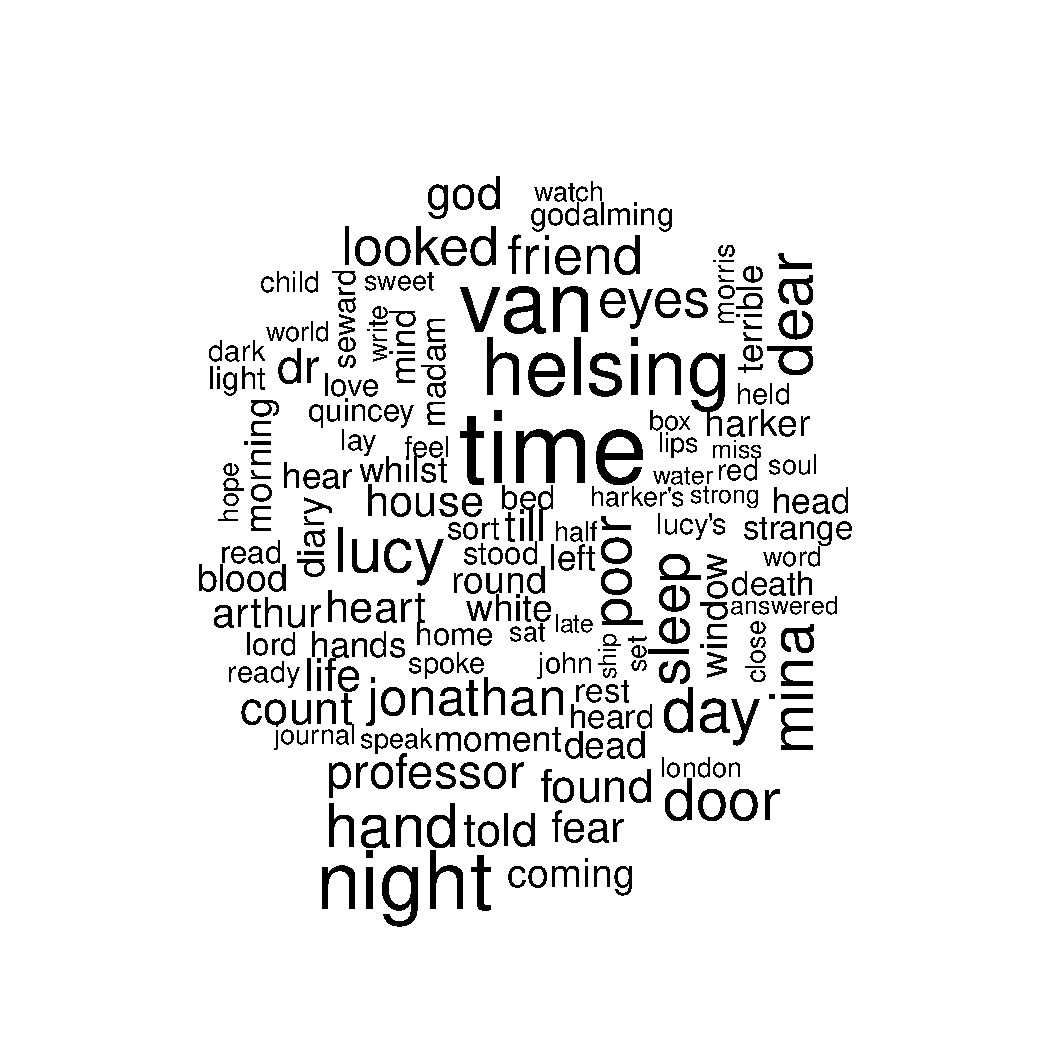
\includegraphics[width=\maxwidth]{figure/unnamed-chunk-5-1} 

\end{knitrout}

Looks great! Now you can try it with a different book to see the main aspects of the novel.

\bibliographystyle{apa}
\bibliography{article}
\nocite{*}

\end{document}
